\begin{figure}[h]
    \centering
    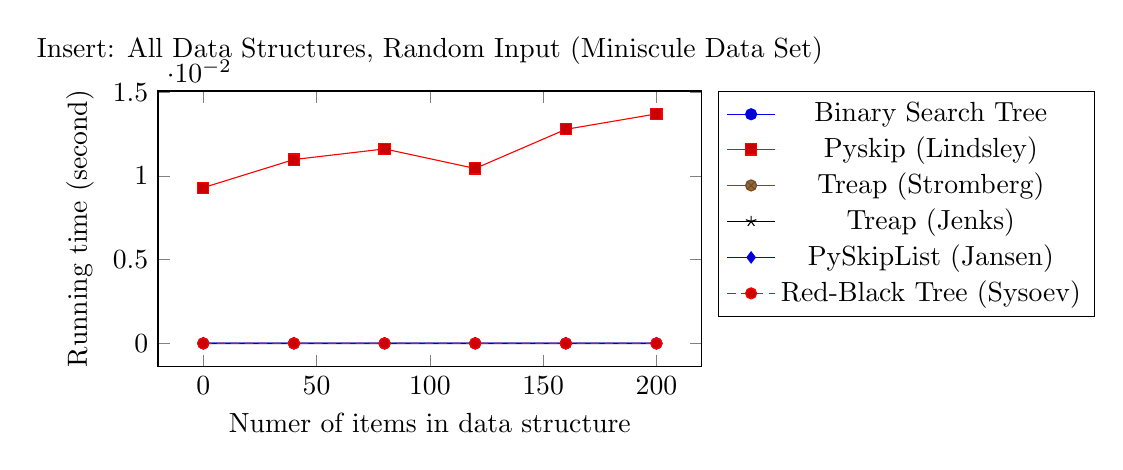
\begin{tikzpicture}
        \begin{axis}[
            xlabel={Numer of items in data structure},
            ylabel={Running time (second)},
            title={Insert: All Data Structures, Random Input (Miniscule Data Set)},
            width=0.7\textwidth,
            height=2in,
            legend pos=outer north east
        ]
		\addplot coordinates {
			(0, 6.655974942226805e-06)
			(40, 6.415034672713204e-06)
			(80, 6.746327543183383e-06)
			(120, 6.776445076894788e-06)
			(160, 6.927032745274176e-06)
			(200, 6.68609247593821e-06)
		};
		\addplot coordinates {
			(0, 0.009299511343016143)
			(40, 0.010977630201862886)
			(80, 0.01161118264025358)
			(120, 0.010444248680475532)
			(160, 0.012779200831243998)
			(200, 0.013700104658429524)
		};
		\addplot coordinates {
			(0, 5.451273595191708e-06)
			(40, 6.083741802243025e-06)
			(80, 4.939275522630737e-06)
			(120, 6.113859336132066e-06)
			(160, 5.119980724721529e-06)
			(200, 4.4573949839588066e-06)
		};
		\addplot coordinates {
			(0, 2.8310481654969523e-06)
			(40, 2.3190500931136173e-06)
			(80, 2.1383448908451897e-06)
			(120, 2.2889325594022126e-06)
			(160, 2.0781098236000163e-06)
			(200, 2.16846242473423e-06)
		};
		\addplot coordinates {
			(0, 2.035945276439577e-05)
			(40, 1.9365574153162868e-05)
			(80, 1.6895936391847498e-05)
			(120, 1.9516161821542254e-05)
			(160, 1.7648874733744434e-05)
			(200, 1.867287087868874e-05)
		};
		\addplot coordinates {
			(0, 6.655974942226805e-06)
			(40, 5.511508662614517e-06)
			(80, 5.9632716677526785e-06)
			(120, 5.692213864527673e-06)
			(160, 5.6319787972824996e-06)
			(200, 5.481391128903112e-06)
		};
        \legend{Binary Search Tree, Pyskip (Lindsley), Treap (Stromberg), Treap (Jenks), PySkipList (Jansen), Red-Black Tree (Sysoev)}
        \end{axis}
    \end{tikzpicture}
    \caption{Average of 10 operations, benchmarked every 40, starting at 0.}
\end{figure}